\documentclass[a4paper,12pt]{article}
\usepackage{graphicx}
\usepackage[utf8]{inputenc}  
\usepackage[T1]{fontenc}
\usepackage{gensymb}

\usepackage{helvet}%Police Arial
\renewcommand{\familydefault}{\sfdefault}

\usepackage[top = 1cm, bottom = 2cm, left = 1cm, right = 1cm]{geometry}
\usepackage{titlesec}
\setcounter{secnumdepth}{4}
\usepackage{xcolor}
\usepackage{amssymb} %double flèche de réaction
\usepackage{xtab}%tableau sur plusieurs pages
\usepackage{esvect}%grands vecteurs

 \usepackage[version=4]{mhchem} %equations chimiques

\usepackage{array}
\usepackage{chemfig}
\usepackage{multirow}
\usepackage{sectsty}
\usepackage{caption}
\usepackage{amsmath}
\usepackage{amssymb}
\usepackage[cal=boondoxo]{mathalfa} 
\usepackage{enumitem}
\usepackage{lastpage}
\usepackage{tcolorbox}
\usepackage{siunitx}
\sisetup{
    detect-all,
    output-decimal-marker={,},
    group-minimum-digits = 3,
    group-separator={~},
    number-unit-separator={~},
    inter-unit-product={~}
} 
\usepackage{tikz}

\graphicspath{ {/home/remy/Documents/Enseignement/2022/Tspe/C6/Ressources/} }

\sectionfont{\fontsize{14}{8}\selectfont}
\renewcommand{\thesection}{\arabic{section}.}
\renewcommand{\thesubsection}{\hspace{1cm}\alph{subsection}.}

\title{\vspace{-1cm}\large 
	\begin{tabular}{|>{\centering}m{5cm}|>{\centering}m{8cm}|>{\centering\arraybackslash}m{4cm}|}
	\hline
	 Tle Spé & \textbf{\textsc{Devoir surveillé 3}} &  \\
	\hline
	\end{tabular}}
\date{}

\newpagestyle{mystyle}{%
\setfoot{}{\thepage\,$|$\,\pageref{LastPage}}{}
}
\renewpagestyle{plain}{%
\setfoot{}{\thepage\,$|$\,\pageref{LastPage}}{}
}

\pagestyle{mystyle}

\newenvironment{itemize*}%
  {\begin{itemize}[label=$-$]%
    \setlength{\itemsep}{0pt}%
    \setlength{\parskip}{0pt}}%
  {\end{itemize}}

\newenvironment{itemize**}%
  {\begin{itemize}[label=]%
    \setlength{\itemsep}{0pt}%
    \setlength{\parskip}{0pt}}%
  {\end{itemize}}

\renewcommand{\tablename}{Tableau}
  
  
\begin{document}
\maketitle
\vspace{-2.5cm}

\section*{Exercice 1 : Pluton et Charon}
Pluton a été découverte par l'astronome Clyde W. Tambaugh, le 18 février 1930, après de longs mois d'observations. Pendant 66 ans, elle fut considérée comme la neuvième planète du système solaire. Cependant, depuis une trentaine d'année, des objets semblables à Pluton de par leur taille et leur masse ont été découverts obligeant l'union astronomique internationale (UAI) à redéfinir la notion de "planète".\\
Depuis Août 2006, Pluton est classée parmi les planètes aines. Jusqu'en 1978, année de découverte du premier satellite naturel Charon, la masse de Pluton n'était pas connue avec exactitude.\\
\textbf{Données :}
\begin{itemize*}
	\item $G$ = \num{6,673e-11} \unit{\meter\cubed \per \kilo\gram \per\second\squared}
	\item 1 année sidérale = 365,2564 jours solaires moyens
	\item 1 jour solaire moyen a une durée égale à \num{86400} \unit{\second}
\end{itemize*}
\textbf{Les caractéristiques de Pluton et de Charon sont données ci-après :}
\begin{table}[h!]
\caption{\label{Tableau1}\textbf{Caractéristiques de Pluton}}
\begin{tabular}{|>{\centering}m{9cm}|>{\centering\arraybackslash}m{9cm}|}
\hline Rayon à l'équateur (\unit{\kilo\meter}) & Distance moyenne au Soleil (\unit{\kilo\meter})\\
\hline \num{1,15e3} & \num{5,91e9}\\
\hline
\end{tabular}
\end{table}

\begin{table}[h!]
\caption{\label{Tableau2}\textbf{Caractéristiques de Charon}}
\begin{tabular}{|>{\centering}m{3.3cm}|>{\centering}m{3.3cm}|>{\centering}m{3.3cm}|>{\centering}m{3.3cm}|>{\centering\arraybackslash}m{3.3cm}|}
\hline Masse (\unit{\kilo\gram}) & Rayon à l'équateur (\unit{\kilo\meter}) & Période de rotation propre (en jours solaires) & Période de révolution autour de Pluton (en jours solaires) & Distance moyenne au centre de Pluton (\unit{\kilo\meter})\\
\hline \num{1,61e21} & \num{6,03e2} & \num{6,387}& \num{6,387} & \num{1,94e4}\\
\hline
\end{tabular}
\end{table}

L'objectif de cet exercice est de déterminer la masse de Pluton en utilisant deux hypothèses qui conduiront à deux valeurs de cette masse notée $M_{P1}$ et $M_{P2}$. Les parties A et B de cet exercice sont indépendantes.

\subsection*{Partie A : Généralités}
	\begin{enumerate}
	\item Quelles sont les deux conditions nécessaires pour observer un mouvement circulaire uniforme ?
	\item La figure suivante représente deux corps $A$ et $B$ à géométrie sphérique et homogènes en masse, de centres de gravité respectifs $O_A$ et $O_B$. $\vec{u}$ est un vecteur unitaire.\\
	La distance entre les deux centres de gravité est notée $d$.
	La masse du corps A est notée $M_A$ et celle du corps B notée $M_B$.\\
	Donner l'expression vectorielle de la force d'interaction gravitationnelle $\vv{F_{A\rightarrow B}}$ exercée par le corps $A$ sur le corps $B$.
	\end{enumerate}
\begin{center}
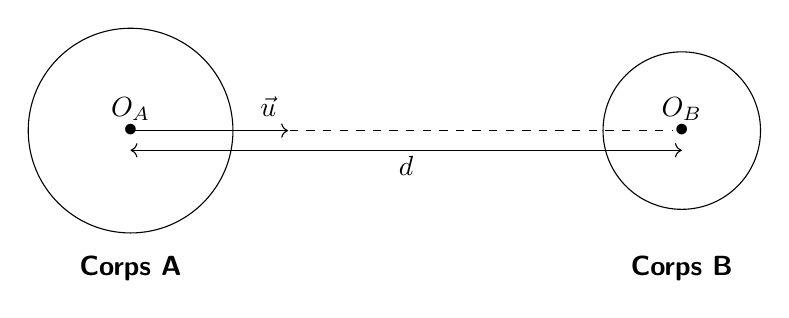
\begin{tikzpicture}
\draw (0,0) circle (1.3) ;
\draw (7,0) circle (1) ;
\node (OA) at (0,0) {};
\draw (OA) node{$\bullet$} node[above]{$O_A$};
\node (OB) at (7,0) {};
\draw (OB) node{$\bullet$} node[above]{$O_B$};
\draw [dashed] (OA) -- (OB);
\draw [<->] (0,-.25) to (7,-.25);
\node (D) at (3.5,-.45) {$d$};
\draw [->] (0,0) to (2,0);
\node (U) at (1.75,.3){$\vec{u}$};
\node (CA) at (0,-1.75) {\textbf{Corps A}};
\node (CA) at (7,-1.75) {\textbf{Corps B}};
\end{tikzpicture}
\end{center}

\subsection*{Partie B : Étude du système Pluton-Charon}
Le référentiel attaché à Pluton est appelé référentiel plutonocentrique que l'on considère galiléen. Les corps célestes Pluton et Charon sont à géométrie sphérique et à répartition uniforme de masse. On néglige toutes les interactions autres que les interactions entre Pluton et Charon.\\
On notera $M_{P1}$ la masse de Pluton, $M_c$ la masse de Charon, $P$ et $C$ les centres de gravité respectifs de Pluton et de Charon.\\
On fera dans un premier temps l'hypothèse que la masse de Charon est négligeable devant celle de Pluton.\\
Le centre de gravité de Charon décrit une trajectoire circulaire de rayon $R$ autour de Pluton. Cette trajectoire est représentée sur la figure ci-dessous. On admet que cette trajectoire est plane.
\begin{center}
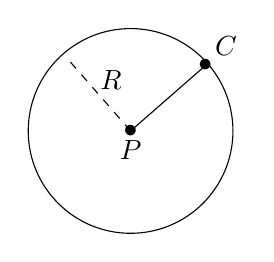
\begin{tikzpicture}
\draw (0,0) circle (1.3) ;
\node (P) at (0,0) {};
\draw (P) node{$\bullet$} node[below]{$P$};
\node (C) at (.95,.83) {};
\draw (C) node{$\bullet$} node[above right]{$C$};
\draw (0,0) -- (.95,.83);
\node (R) at (-.25,.65) {$R$};
\draw [dashed] (0,0) -- (-.83,.95);
\end{tikzpicture}
\end{center}
\begin{enumerate}
	\item Pluton met 6,387 jours solaires pour faire un tour sur elle-même et 248 années sidérales pour effectuer un tour autour du Soleil.\\
	Quelle est la période de révolution de Pluton, dans les unités du système international ? Justifier la réponse.
	\item En appliquant la seconde loi de Newton au centre d'inertie de Charon, en déduire les caractéristiques (direction, sens, norme) du vecteur accélération $\vec{a}$ du centre d'inertie de Charon. La norme sera exprimée en fonction des connées de l'énoncé.
	\item Vérifier que le mouvement circulaire uniforme est une solution de la relation établie à la question précédente et montrer alors que la vitesse du centre d'inertie de Charon est $v = \sqrt{\dfrac{G \cdot M_{P1}}{R}}$
	\item Établir l'expression de la période de révolution $T$ de Charon autour de Pluton.
	\item Déduire des deux questions précédentes la relation suivante : $\dfrac{T^2}{R^3} = \dfrac{4\pi^2}{G\cdot M_{P1}}$
	\item À l'aide de la question précédente, expliquer ce qui a permis, à partir de 1978, de déterminer la masse de Pluton.
	\item En utilisant les tableaux de données et la question 5, calculer la masse $M_{P1}$ de Pluton.
	\item En réalité, la masse de Charon n'est pas négligeable devant celle de Pluton. On cherche donc à calculer la masse de Pluton, notée $M_{P2}$ en tenant compte de cette nouvelle hypothèse. On trouve alors que : $\dfrac{T^2}{R^3} = \dfrac{4\pi^2}{G\cdot M_{P1}+M_C}$.
	En déduire la masse $M_{P2}$ de Pluton.
	\item La valeur admise de la masse de Pluton est \num{1,32e22} \unit{\kilo\gram}. Discuter de la pertinence de l'hypothèse formulée à la question précédente.
\end{enumerate}
\newpage
\section*{Exercice 2 : Éruption de la montagne pelée en 1902}

Il s’agit dans cet exercice de chercher l’ordre de grandeur des vitesses d’éjection des blocs de matière émis lors de cette éruption volcanique et de déterminer l’altitude maximale atteinte par un bloc dans une situation donnée.
On considère, dans le référentiel terrestre supposé galiléen, un bloc de matière de masse $m$. Ce bloc est assimilé à un point matériel.\\
Le repère d’étude ($O$, $\vec{i}$, $\vec{k}$) est choisi de telle sorte que le vecteur vitesse initiale $\vec{v_0}$ soit dans le plan $xOz$, incliné d’un angle $\alpha$ par rapport à l’axe ($Ox$). L’origine des dates est l’instant où le bloc quitte le point $O$.
\begin{center}
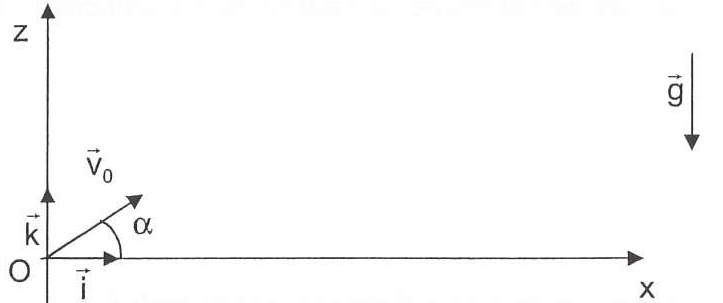
\includegraphics[scale=.45]{Ressources/TSPE_C6_Evaluation_Fig2.png}
\end{center}
Dans tout l’exercice, on néglige la poussée d’Archimède et les forces de frottements dues à l’air. La valeur de l’intensité de pesanteur $g$ est prise égale à \num{9,8} \unit{\meter\per\second \squared}
\begin{enumerate}
	\item \underline{Équations horaires du mouvement}
	\begin{enumerate}
		\item Pourquoi peut on dire que le bloc est en chute libre ?
		\item En appliquant la seconde loi de Newton, établir la relation entre le vecteur accélération $\vec{a}$ du centre d’inertie du bloc et le vecteur champ de pesanteur $\vec{g}$, puis donner l’expression des composantes $a_x(t)$ et $a_z(t)$ dans le repère d’étude.
		\item En déduire les expressions littérales $v_x(t)$ et $v_z(t)$ des composantes horizontales et verticales du vecteur vitesse du bloc.
		\item Montrer que les expressions des équations horaires du mouvement $x(t)$ et $z(t)$ sont : 
		\begin{eqnarray}
		x(t) = (v_0 \cdot \cos{\alpha})\cdot t \nonumber \\
		z(t) = -\dfrac{1}{2} \cdot g \cdot t^2 + (v_0 \cdot \sin{\alpha}) \cdot t \nonumber
		\end{eqnarray}
	\end{enumerate}
	\item \underline{Bloc éjecté du cratère avec une vitesse initiale $\vec{v_0}$.}\\
	Les observations les plus directes concernent la hauteur h atteinte par de gros blocs lancés verticalement lors de l’éruption. De cette hauteur h, on tire la vitesse : $\sqrt{2 \cdot g \cdot h}$.\\
L’épouvantable éruption de la Montagne Pelée n’a réussi à lancer des pierres de volume un peu considérables qu’à 400 m. Ici le vecteur vitesse initiale est dirigé verticalement vers le haut.
	\begin{enumerate}
		\item À partir des réponses aux questions 1.c. et 1.d., préciser les expressions de $v_x(t)$, $v_z(t)$, $x(t)$ et $z(t)$ dans la situation étudiée.
		\item À partir de l'expression de $v_z(t)$, déterminer l'expression de la date $t_S$ à laquelle l'altitude maximale $h$ est atteinte.
		\item En déduire que l'expression de la vitesse initiale est $\sqrt{2 \cdot g \cdot h}$.
		\item Calculer la valeur de $v_0$ si l'éjection atteint $h$ = \num{400} \unit{\meter}.
	\end{enumerate}
\end{enumerate}
\end{document}
